% Enable warnings about problematic code
\RequirePackage[l2tabu, orthodox]{nag}

\documentclass{resources/WeSTassignment}
\usepackage{tabularx}
\usepackage{booktabs}
\usepackage[utf8]{inputenc}
\usepackage{amsmath}
\usepackage{graphics}
\usepackage{graphicx}
\usepackage{changebar}
\usepackage{latexsym}
\usepackage{stmaryrd}
\usepackage{booktabs}
\usepackage{amsmath}
\usepackage{wasysym}
\usepackage[export]{adjustbox}
\usepackage[thinlines]{easytable}
\usepackage{framed}
\usepackage{color}
\usepackage{footnote}
\usepackage{listings}
\usepackage{framed}
\usepackage{tikz}

%\solutiontrue
% The lecture title, e.g. "Web Information Retrieval".
\lecture{Introduction to Web Science}
% The names of the lecturer and the instructor(s)
\author{%
  PD Dr. Matthias~Thimm\\{\normalsize\mailto{thimm@uni-koblenz.de}} \and
  Ipek Baris Schlicht\\{\normalsize\mailto{ibaris@uni-koblenz.de}} \and
  Kenneth Skiba\\{\normalsize\mailto{kennethskiba@uni-koblenz.de}}
}
% Assignment number.
\assignmentnumber{3}
% Institute of lecture.
\institute{%
  Institute of Web Science and Technologies\\%
  Department of Computer Science\\%
  University of Koblenz-Landau%
}
% Date until students should submit their solutions.
\datesubmission{01.12.2020, CEST 23:59}

% Specify bib file location.
\addbibresource{bibliography.bib}

\begin{document}

\maketitle

\section{Recursive Query: DNS \hfill{20 Points}}
For this task we will extend the routing table from the fourth task on Assignment 1.

In the following schema rectangles represent the networks, with there name inside. The circles are the routers. An edge between a router and a network means, that a router is part of this network and has the MAC address written at the edge in blue, while the interface is written in black.

In the routing table below you find an entry for every router. One entry in the routing table of a router contains a three tuple of Destination, Next Hop and Interface. 
\begin{figure}[h]
    \centering
    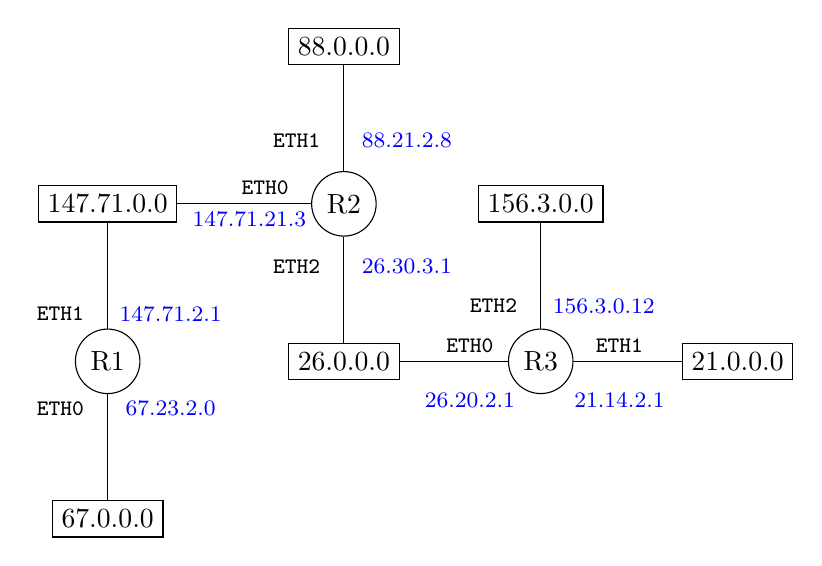
\begin{tikzpicture}
\node[draw, rectangle](C1) at (0,0) {67.0.0.0};
\node[draw, rectangle](C2) at (0,4) {147.71.0.0};
\node[draw, rectangle](C3) at (3,6) {88.0.0.0};
\node[draw, rectangle](C4) at (3,2) {26.0.0.0};
\node[draw, rectangle](C5) at (8,2) {21.0.0.0};
\node[draw, rectangle](C6) at (5.5,4) {156.3.0.0};

\node[draw, circle](R1) at (0,2) {R1};
\node[draw, circle](R2) at (3,4) {R2};
\node[draw, circle](R3) at (5.5,2) {R3};

\draw[-](C1) to (R1);
\node (R1_eth0) at (-0.6,1.4) {\texttt{\footnotesize{ETH0}}};
\node (R1_mac0) at (0.8,1.4) {\textcolor{blue}{\footnotesize{67.23.2.0}}};
\draw[-](R1) to (C2);
\node (R1_eth1) at (-0.6,2.6) {\texttt{\footnotesize{ETH1}}};
\node (R1_ma1) at (0.8,2.6) {\textcolor{blue}{\footnotesize{147.71.2.1}}};
\draw[-](C2) to (R2);
\node (R2_eth0) at (2,4.2) {\texttt{\footnotesize{ETH0}}};
\node (R2_mac0) at (1.8,3.8) {\textcolor{blue}{\footnotesize{147.71.21.3}}};
\draw[-](R2) to (C3);
\node (R2_eth1) at (2.4,4.8) {\texttt{\footnotesize{ETH1}}};
\node (R2_ma1) at (3.8,4.8) {\textcolor{blue}{\footnotesize{88.21.2.8}}};
\draw[-](R2) to (C4);
\node (R2_eth2) at (2.4,3.2) {\texttt{\footnotesize{ETH2}}};
\node (R2_ma2) at (3.8,3.2) {\textcolor{blue}{\footnotesize{26.30.3.1}}};
\draw[-](C4) to (R3);
\node (R3_eth0) at (4.6,2.2) {\texttt{\footnotesize{ETH0}}};
\node (R3_mac0) at (4.6,1.5) {\textcolor{blue}{\footnotesize{26.20.2.1}}};
\draw[-](R3) to (C5);
\node (R3_eth1) at (6.5,2.2) {\texttt{\footnotesize{ETH1}}};
\node (R3_mac1) at (6.5,1.5) {\textcolor{blue}{\footnotesize{21.14.2.1}}};
\draw[-](R3) to (C6);
\node (R3_eth2) at (4.9,2.7) {\texttt{\footnotesize{ETH2}}};
\node (R3_mac2) at (6.3,2.7) {\textcolor{blue}{\footnotesize{156.3.0.12}}};
\end{tikzpicture}
    \caption{Routing schematic representation}
    \label{fig:schematic_routing}
\end{figure}

\begin{table}[h]
    \centering
    \scalebox{0.8}{
\begin{tabular}{|l|l|l|l|l|l|l|l|l|}
\hline
\multicolumn{3}{|c|}{Router 1}        & \multicolumn{3}{c|}{Router 2}         & \multicolumn{3}{c|}{Router 3}        \\ \hline
Destination & Next Hop    & Interface & Destination & Next Hop    & Interface & Destination & Next Hop   & Interface \\ \hline
67.0.0.0    & 67.23.2.0   & eth0      & 147.71.0.0  & 147.71.21.3   & eth0      & 26.0.0.0  & 26.20.2.1 & eth0      \\ \hline
147.71.0.0    & 147.71.2.1   & eth1      & 88.0.0.0  & 88.21.2.8 & eth1      & 21.0.0.0   & 21.14.2.1  & eth1      \\ \hline
88.0.0.0  & 147.71.21.3 & eth1      & 26.0.0.0    & 26.30.2.1    & eth2      & 88.0.0.0    & 26.30.3.1 & eth0      \\ \hline
26.0.0.0    & 147.71.21.3 & eth1      & 67.0.0.0    & 147.71.2.1 & eth0      & 147.71.0.0  & 26.30.3.1  & eth0      \\ \hline
21.0.0.0  & 147.71.21.3   & eth1      & 21.0.0.0    & 26.20.2.1 & eth2      & 67.0.0.0    & 26.30.3.1  & eth0      \\ \hline
156.3.0.0  & 147.71.21.3   & eth1      & 156.3.0.0    & 26.20.2.1 & eth2      & 156.3.0.0    & 156.3.0.12  & eth2      \\ \hline
\end{tabular}
}
    \caption{Routing table}
    \label{sol:tab:routing_table}
\end{table}

Let us assume a client with the following IP address 67.4.5.2 wants to resolve the following domain  \texttt{subdomain.webscienceexample.com} using the DNS.

You can further assume the root name server has the IP address of 88.8.2.1 and the name-server for \texttt{com} has the IP address 156.3.20.2. 
Finally the domain is handled by a name server with the IP of 21.155.36.7.

Please explain how the traffic flows through the network in order to resolve the recursive DNS query. You can assume ARP tables are cached so that no ARP-requests have to be made. \\ \\ \textbf{Solution:}
\begin{enumerate}
\item The client with IP address \textbf{67.4.5.2} reaches the router\textbf{R1} in order to issue a \textbf{DNS request} to the root name server with the destination IP address \textbf{88.8.2.1}. Now the router \textbf{R1} looks into its routing table and finds the next hop to be \textbf{147.71.2.3} in order to reach the network \textbf{88.0.0.0} and reaches the Router \textbf{R2} . Now since router \textbf{R2} is directly connected to the network \textbf{88.0.0.0},it delivers the \textbf{IP packet} requesting the IP address of \textbf{subdomain.webscienceexample.com} to the root name server at   \textbf{88.8.2.1} .
\item The root name server responds with the referral to top level domain \textbf{.com} with IP address \textbf{156.3.20.2}. Now this IP packet is routed back from the destination \textbf{88.8.2.1} to client at \textbf{67.4.5.2}. This packet from router \textbf{R2} reaches router \textbf{R1} with the next hop \textbf{147.71.2.1} . Since the network \textbf{67.0.0.0} is directly connected to router \textbf{R1}. The packet gets delivered to the client at \textbf{67.4.5.2}.
\item The client sends a another DNS request to the name server with IP \textbf{156.3.20.2}. This IP packet reaches router \textbf{R1}.The router repeats the process of looking into its table and routes the packet to router \textbf{R2} through next hop \textbf{147.71.21.3}. Now the router 2 looks into its table and routes the packet to router \textbf{R3} through next hop \textbf{26.20.2.1}.Router \textbf{R3} delivers the IP packet to the name server at destination \textbf{156.3.20.2}. 
\item The name server now responds with an IP packet consisting of the address of the name server \textbf{webscienceexample.com} to the client which is now acting as the destination at \textbf{67.4.5.2}. This packet is routed from \textbf{R3} to router \textbf{R2} with the hop \textbf{26.30.3.1}. The packet from router \textbf{R2} reaches router \textbf{R1} through next hop \textbf{147.71.2.1}.The router \textbf{R1} delivers the packet to the client.
\item Now the client sends the request to the name server \textbf{webscienceexample.com} at destination with IP \textbf{21.155.36.7}. This packet is routed from \textbf{R1} to \textbf{R2} through next hop \textbf{147.71.21.3}. The packet is routed from \textbf{R2} to \textbf{R3} through next hop \textbf{26.20.2.1}. The request is delivered to the name server through \textbf{R3}.
\item The name server sends an IP packet with requested information to the client at destination \textbf{67.4.5.2}. This packet is routed from \textbf{R3} to router \textbf{R2} with the hop \textbf{26.30.3.1}. The packet from router \textbf{R2} reaches router \textbf{R1} through next hop \textbf{147.71.2.1}.The router \textbf{R1} delivers the packet to the client.

\end{enumerate}

	
\section{Internet Architecture \hfill{20 Points}}
\begin{enumerate}
    \item Explain in your own words the four layer of the Internet architecture.
    \item Formulate an example to show the usage of the aforementioned layers.
\end{enumerate}

\section{World Wide Web \hfill{14 Points}}
\begin{enumerate}
    \item Name two different motivation points for the construction of the world wide web and explain why these points were necessary.
    \item Describe five design principles of the world wide web with your own words. 
\end{enumerate}

\section{Python Programming \hfill{26 points}}
\subsection{URL Parser \hfill{13 points}\label{url_parser}}
Write a Python script called as \texttt{urlparser.py}. The script parses an url into the segments that are explained in the lecture \textbf{Internet vs WWW}, and additionally extracts top-level domains as one segment \footnote{https://en.wikipedia.org/wiki/Top-level\_domain}. When you execute the script (e.g \texttt{python -m urlparser https://west.uni-koblenz.de/studying/ws2021}) at the command-line, a dictionary containing the url and its segments should be returned. For the optional parts, you may use \texttt{None} values. 

Take a screenshot of the terminal output of your script for the following URLs
\begin{enumerate}
    \item \url{https://www.facebook.com/photo.php?fbid=2068026323275211&set=a.269104153167446&type=3&theater}
    \item \url{http://www.blog.google.uk:1000/path/to/myfile.html?key1=value1&key2=value2#InTheDocument}
    \item \url{https://www.overleaf.com/9565720ckjijuhzpbccsd#/347876331/}
    \item \url{ftp://root@west.uni.koblenz.de}
    \item \url{https://west.uni-koblenz.de/studying/ws2021}
    
\end{enumerate}

You are not allowed to use any specific libraries that help in url parsing and regular expressions. 

\subsection{Simple HTTP Web Client \hfill{13 points}}
You are asked to write a simple HTTP client (\textbf{httpclient.py})
that takes a URL and is able to download that webpage from the World Wide Web and store it on your hard drive (in the same
directory as your python code is running). The program should also print out the complete
HTTP header of the response and store the header in a \textit{separate file}.


You are allowed to use 1) socket, 2) \texttt{urlparser.py} that you implement for the Question~\ref{url_parser} 3) sys for reading input from the command-line. 


Run your code on the following urls. Analyse the responses: (1) what is the response code (2) explain briefly why does the website respond with that code? 
\begin{enumerate}
\item 
\url{http://example.com}
\item\url{http://example.com/test.html}
\item 
\url{https://west.uni-koblenz.de/research/projects}
\end{enumerate}

\textbf{Warning:} Please don't make consecutive calls to the websites.
\end{document}